\documentclass[12pt,hidelinks]{article}
\usepackage{graphicx,hyperref,amsmath,natbib,bm,url}
\usepackage{microtype,todonotes}
\usepackage[a4paper,text={14.5cm,23.2cm},centering]{geometry}
\usepackage[compact,small]{titlesec}
\usepackage[utf8]{inputenc}
\usepackage[nottoc,numbib]{tocbibind}

\clubpenalty = 10000
\widowpenalty = 10000
\usepackage[T1]{fontenc}
\hypersetup{
     colorlinks   = true,
     citecolor    = black,
     linkcolor    = black,
     urlcolor     = black
}
\renewcommand{\figurename}{Figur}
\renewcommand{\contentsname}{Indholdsfortegnelse}

\begin{document}
    \sloppy
    \titleGM
	\newpage
	\tableofcontents
	\newpage
	\section{Indledning}
	Selvkørende biler er meget oppe i medierne i disse dage, og man kan spørge sig selv hvorfor dette er tilfældet. Hvis man spørger producenterne af teknologien, får man svaret; at de selvkørende biler vil gøre trafikken mere sikker, samt vil udnytte vejene meget bedre \cite{GOOG_SITE}. I den forbindelse spurgte vi os selv: ``Jamen hvis de har så mange tilsyneladende fordele, hvorfor er bilerne så ikke godkendt til at køre rundt på vejene?''. 

Det er relevant at undersøge, om der er et ønske fra befolkningen om at få de selvkørende biler, da de også er med til at drive forskningen frem ved at skabe efterspørgsel efter teknologien. Efterspørgslen vil presse politikerne til at tage stilling til, om bilerne skal godkendes. Forskere fra Transportation Research Institute hos University of Michigan har undersøgt, hvor stor en del af befolkningen ønsker de selvkørende biler\cite{UMTRI}. Svaret var at 60\% ud af de 505 spurgte billister, har et ønske om enten delvist selvkørende biler eller helt selvkørende biler. De delvist selvkørende biler er typen som Google er ved at udvikle hvor føreren kan overtage kontrollen, hvorimod de fuldstændigt selvkørende biler ikke har brug for en fører.

Den store efterspørgsel efter de selvkørende biler, giver god grund til at undersøge dette initierende problem, og finde årsagerne til den manglende godkendelse af bilerne.
	\section{Problemanalyse}
	\textit{I dette afsnit vil vi undersøge hvilke problemer der står i vejen for at biler bliver godkendt til at køre på vejene. Vi har inddelt vores problemanalyse i to hovedpunkter, de teknologiske- og de samfundsmæssige udfordringer. På denne måde vil vi forsøge at få et overblik over problemet, og lokalisere de steder, hvor man kunne forbedre systemet så bilerne kan blive godkendt.}
	\subsection{Begrebsforklaringer}
	\subsubsection{Niveauer af automatisering af biler}
SAE International, tidligere Society of Automotive Engineers, er en organisation som fastsætter nye standarder indenfor automobil-industrien. Ifølge deres standard J3016 udgivet januar 2014, kan biler inddeles i 6 niveauer af automatisering, fra niveau 0 hvor der ingen automatisering er, til niveau 5 hvor alle funktioner i bilen er automatiseret \cite{SAE_J3016}. 

De fem niveauer kan beskrives som følger:

\begin{description}
	\item[Niveau 0] betyder ingen automatisering. Det vil sige at det er føreren af bilen der tager stilling til alle situationer, og selv har den fulde kontrol over bilen.
	\item[Niveau 1] betyder at bilen har kontrol over enten styring eller acceleration/deacceleration, mens føreren styrer de andre opgaver. Det er stadig føreren, der skal være opmærksom og fortælle bilen hvad den skal gøre. Dette niveau kan f.eks. være en fartpilot, hvor føreren blot bestemmer en fart, og så accelererer bilen op til denne hastighed, og holder derefter farten. 
	\item[Niveau 2] betyder at bilen kan styre bilen uden føreren, dog kun i nogle meget begrænsede tilfælde. Det er stadig føreren af bilen der skal holde øje med omgivelserne. Det vil sige at niveau 2 er delvis automatisering, altså automatisering af nogle få og specifikke opgaver i kørslen.
	\item[Niveau 3] er hvor man kan sige at en bil er selvkørende. Fra niveau 3 og fremefter, er det systemet der holder øje med omgivelserne, og analyserer forhindringer som bilen skal tage stilling til. På niveau 3 skal der dog være en fører af bilen der sidder klar til at overtage kontrollen af bilen, hvis bilen ikke kan genkende den situation den befinder sig i.
	\item[Niveau 4] og fremefter, har selv en fallback løsning hvis bilen oplever en ukendt situation. Dog gælder det stadig for niveau 4 at bilen ikke kan køre i alle situationer, og at brugeren stadig skal overtage i nogle bestemte situationer. Altså er bilen kun selvkørende i nogle scenarier, men i disse scenarier har den ikke brug for brugerens input.
	\item[Niveau 5] er fuld automatisering af bilen, og bilen har ikke længere brug for en fører af bilen. Den leverer selv fallback løsninger, og kan køre i alle kørselsscenarier. Dette er niveauet hvor man ikke har brug for et kørekort for at køre bilen, da den selv styrer alt, fra du sætter dig ind i bilen og til at du er fremme.
\end{description}

Den virksomhed som er længst med udviklingen af selvkørende biler, og får mest opmærksomhed i medierne er Google. Googles projekt for selvkørende biler, er lige nu en niveau 3 selvkørende bil, da der bag rattet skal sidde en billist med kørekort, klar til at overtage styringen hvis der går noget galt for programmet. Det vil sige at den AI som styrer bilen holder styr på omgivelserne og kører potentielt uden brug for billisten, men kan også advare billisten om at denne skal overtage styringen af bilen.

Googles selvkørende bil virker ved at den på taget af bilen har en laser som bruges til at scanne omgivelserne, og tegner et 3D kort over omgivelserne. Teknologien der bruges til dette hedder Lidar som er en sammentrækning af ordene ``light'' og ``radar'', virker ved at laseren peger på et objekt og analyserer det lys der kommer tilbage. Jo længere tid det tager for lyset at komme tilbage, jo længere er objektet fra laseren. Ved at gøre dette på omgivelserne omkring bilen, kan der tegnes et detaljeret 3D kort over bilens position. Desuden bruger bilen også radarer samt kameraer til at få et overblik over hvor den befinder sig. Alle oplysninger fra disse sensorer behandles af en computer som så ved hjælp af kunstig intelligens kan beslutte hvordan den skal reagere på dens situation. Den software som behandler dataet og træffer beslutninger hedder Google Chauffeur.

\subsubsection{Kunderne til de selvkørende biler}
Grunden til at det er relevant at kigge på disse selvkørende biler og deres udfordringer, er at der er mange potentielle kunder for denne teknologi. Når teknologien har mulighed for at blive udbredt mange steder, er det vigtigt at kende til de fordele og ulemper teknologien bringer, inden teknologien tages i brug.

Netop denne teknologi har potentiale til at blive udbredt på markedet, da en selvkørende bil eksempelvis vil være i stand til at spare mange mennesker tid hver morgen. Tiden i myldretrafikken ville da kunne benyttes på at arbejde, frem for at køre bil. Desuden lover producenterne af disse biler, også at disse biler vil øge trafiksikkerheden \cite{GOOG_SITE}, hvilket ville være endnu et incitament for en privat kunde at købe en sådan bil.

Udover den åbenlyse kunde i form af private mennesker er der også virksomheder, som ville kunne tænkes at bruge denne teknologi i deres forretningsmodel. Dette kunne f.eks. være et taxi-selskab der nu ikke nødvendigvis har brug for chauffører, da en computer nu kan styre bilen i stedet. Busser kunne også være et område hvor man kunne benytte denne teknologi. Man kunne her igen spare lønnen til chaufføren, og virksomhederne ville kunne spare penge.

Som man kan se ud fra de ovennævnte punkter, er der mange muligheder for hvordan denne teknologi vil kunne blive brugt at både private mennesker og virksomheder. Når en teknologi bliver spredt i verden på denne måde, bliver vi nødt til at kigge nærmere på sikkerheden omkring den. Vi vil derfor i de følgende afsnit fokusere på om teknologien er klar til markedet endnu, samt kigge på om det er muligt at sikre sig at disse biler er sikret over for hackere, der ønsker at skaffe kontrol over din bil. Et andet punkt som vi vil undersøge, er om hvilke indflydelse det vil have overfor vores hverdag, hvis disse biler blev en realitet.

\subsubsection{Producenterne af de selvkørende biler}
Udover kunderne, er der selvfølgelig også en anden gruppe mennesker der ønsker at få disse biler godkendt til vejene, nemlig producenterne af denne. Producenterne af bilerne bruger penge på lobbyister for at sikre sig at bilerne bliver godkendt til vejene\cite{soprweb}. Store bilfirmaer som Toyota, Mercedes og Audi har alle fremvist biler \cite{PopularMechanics} som kan beskrives som selvkørende biler. Disse firmaer har alle udtalt at de vil have biler på vejene med denne teknologi før 2020, og der er dermed sat et kapløb igang om hvem der først får sine biler på markedet. 
	\subsection{Teknologiske}
	I dette delafsnit vil vi kigge nærmere på de teknologiske problemer der er ved at få en selvkørende bil godkendt. Derfor kigger vi både på hvordan bilerne virker, og hvilke svagheder dette har, samt kigger på, hvordan hackning kunne vise sig at være en stor problemstilling inden for de selvkørende biler.
	\subsubsection{Bilernes interaktion med andre mennesker}

I takt med at der kommer flere selvkørende biler på vejene, er der kommet mere lys på de problemer som disse biler har når de interaktioner med omgivelserne. En af de større udfordringer de har mødt, er selve trafikken og alt der hører med til denne. Bilens sensorer gør at den har en større årvågenhed end andre bilister, hvilket faktisk har vist sig at være et problem. Problemet er, at bilens opmærksomhed også sætter den i stor fare for at blive påkørt af en uopmærksom bilist som kommer kørende bagfra. Dette bekræfter Google selv i deres månedlige rapport fra august 2015\cite{GOOG_MONTHLY}. Et eksempel på dette skete på en travl vej i Mountain View Californien, hvor fodgængere kan trykke på en knap, for at få et lys på vejen til at skifte så de kan gå over. Her havde den selvkørende bil opdaget en person ude på dette fodgængerfelt, hvorefter testpersonen i bilen valgte manuelt at bremse, for at sikre at de ikke ville ramme personen. Dog var bilen bag den selvkørende bil ikke lige så vågen, så den endte med at køre op bag i den selvkørende bil. Det skal dog siges at trods den manuelle bremsning af testkøreren, så viste det sig senere at bilen selv ville være stoppet i tide. Dog ville den have kørt noget tættere på fodgængeren, hvilket kunne have virket skræmmende for fodgængeren\cite{GOOG_MONTHLY}. 

En anden udfordring de selvkørende biler har, er at som de er nu, kører ekstremt sikkert. I dette tilfælde skal ordet sikkert ikke tages på en god måde. Den selvkørende bil kan virke som om den er lige lidt for langsom ude af lyskrydset, og som altid sikrer sig at den ikke overstiger fartgrænsen på nogen måde. Dette gør at den ellers travle trafik bliver sinket af de selvkørende biler som er på gaden. Denne form for kørsel ville i princippet ikke være et problem for bilen, men da der ikke er nogen mennesker der kører på helt samme måde, så skaber det som sagt nogle problemer. Et eksempel kunne være som vist på følgende figur.

\begin{figure}[h!]
    \centering
    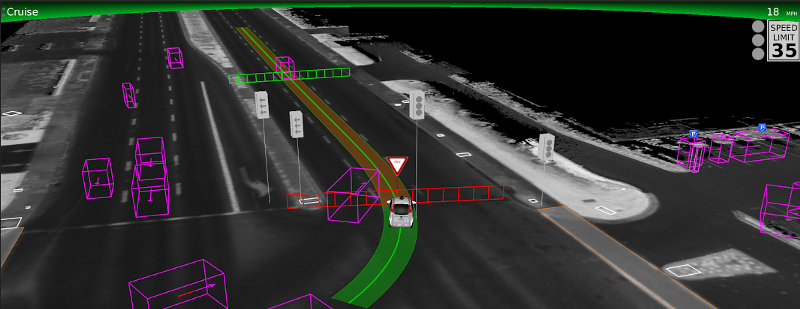
\includegraphics[width=0.8\textwidth]{images/google_vision.png}
    \captionsource{Bilens scan, der viser hvad der er i nærheden. Altså dens syn.}{\url{https://cdn-images-1.medium.com/max/800/0*\_HAJZvL781n19u5z.}}
    \label{fig:car_vision}
\end{figure}

Figuren er taget af bilens syn på omverden under en situation der virker godt som et eksempel på dens kørsel. Her er de lyserøde kasser andre køretøjer, den grønne linje viser bilens planlagte rute, og midt i selve billedet er bilen selv. Men situationen her er, at bilen på den venstre side af den selvkørende bil svinger lidt bredt, da den har overset den selvkørende bil. Hvilket gør at den kommer ind i den selvkørende bils bane. Så i stedet for selv at tage et lidt bredere sving, så vælger den selvkørende bil at bremse ned. Dette tydeliggøres også på figuren, hvor der fremgår et rødt hegn foran bilen, hvilket betyder at bilen bremser\cite{Backchannel}. En af de givne problemer mange byer er begyndt at møde, er at den store mængde mennesker der bor i disse byer, skal selvfølgelig have en form for transport. Dette er så biler, eller offentlig transport. Dette har gjort at selve byernes infrastruktur ikke har kunne følge med alle de mennesker der nu befinder sig på vejene, så den meget øgede trafik har gjort at kørsel i byerne er blevet meget aggresivt, for at komme hurtigere frem. Da tid brugt i trafikken kunne være brugt på en mere produktiv måde\cite{Michelin}. I sådanne et miljø ville den selvkørende bil både være en fordel og en ulempe. Det nemmeste ville selvfølgelig være hvis alle selv havde en selvkørende bil, da hele ruten ville kunne blive kalkuleret, så man ville kunne få en præcis tid for, hvor lang tid ruten ville tage, og man ville kunne lave noget andet samtidigt med at man kørte. Den store ulempe bilen vil have, er at hvis man som den eneste kører rundt i en selvkørende bil i disse områder vil det forstyre trafikken meget. Da de som nævnt tidligere kører meget sikkert, så gør den aggressive kørsel for de andre bilister, at den selvkørende bil vil kunne være en fare for sig selv. Her kunne et eksempel være, at den ikke ville skynde sig over for et gult lys, mens bilisten bag den tænkte at det var nået man godt kunne nå. Hvilket ville resultere i at den selvkørende bil ville blive påkørt bag fra.

En anden situation hvor sådan en bil fejlede i at reagere blev beskrevet af en cyklist i Austin, Texas, hvor han nemlig mødte en sådanne selvkørende bil i et kryds, mens han var på cykel. Cyklisten lavede så det man kalder en track-stand, men han lagde sig ind bag bilen. En track-stand er en teknik man bruger til at holde sig på cyklen når man kører rigtigt langsomt, hvor man så også bevæger styret på cyklen frem og tilbage for at holde balancen. Den selvkørende bil misforstod så denne track-stand for en cyklist der kom kørende bag den og stoppede. Så da bilen kunne se at cyklisten holdt stille kørte den så igen, hvorefter den så stoppede igen fordi cyklisten bevægede styret fra den ene side til den anden. Dette gjorde at bilen stadig ikke var nået ud til midten af krydset efter hele 2 minutters kørsel\cite{VOX}. Det lyder måske ikke af meget, men det er sådanne problemer man er nød til at sikre ikke sker efter bilen er udgivet til private personer, da begge hændelser ville kunne føre til større ulykker, yderligere forsinkelser af trafikken eller fører til personskader. 
	\subsection{Sikkerhedskritisk software}
Ved at køre i de elektroniske køretøjer er der mange sikkerhedsmæssige fordele, i det at mennesker laver fejl som koster mange menneskers liv. Ved at gøre forskellige funktioner elektroniske mindsker man menneskelige fejl. Dog er der visse usikkerheder ved at lægge sin lid til maskinen alene. Usikkerheden ligger blandt andet i, at man som i alle andre elektroniske systemer kan `hacke' sig ind og ændre ved systemet. For eksempel er det muligt, med en relativ simpel teknik at kunne fjernstyre køretøjet. Det gør det muligt for `hackeren', at forstyrre kørselen og gøre det direkte farligt at køre. Dette er heldigvis ikke et udbredt problem endnu.  

Da producenterne gerne vil skabe en illusion om sikkerhed; hvad angår de elektroniske og automatiske køretøjer. Derfor bliver der lagt rigtig meget tid af til forskning i ikke at gøre denne usikkerhed til en virkelighed. Forskningen bliver foretaget af forskellige sikkerhedsforskere, som forsøger at påvise så mange fejl og usikkerheder ved køretøjet som muligt. Dette foregår ved at de selv `hacker' bilerne, og på den måde påviser under kontrollerede forhold, hvilke ricisier der er ved at automatisere flere af køretøjets funktioner.  


Et eksempel er sikkerhedsforskeren Charlie Miller og direktøren for IOactive Chris Valasek som har brugt over et års forskning på at undersøge og påvise hvordan man kan overtage kontrollen af en Jeep ved hjælp af en såkaldt zero-day exploit. Under forsøget opdagede de en fejl ved infotainment systemet, Harman uConnect, at internetforbindelsen igennem netværket Sprint, havde porten 6667 stående åben. Dette gav dem mulighed for at koble sig til bilen via deres smartphone over det cellulære netværk. Charlie og Chris var via en femtocell i stand til at fjernstyre Jeepen helt op til 110km. væk. Under angrebet på Jeepen var de i stand til blandt andet at styre rattet under bakkemanøvre, sætte bremserne ud af funktion og skifte gear, herudover nogle mindre ting som at styre klimaanlægget, sædevarmen, radioen, vinduesviskerne og sprinklervæsken.  

Chris og Charlie har efterfølgende indberettede fejlene de fandt under forskningen til Chrysler og Sprint, som var hurtige til at få rettet fejlene og få lukket den åbne port. Herudover fik Chrysler kaldt de fejlproducerede biler tilbage og fik lavet en opdatering som blev tilgængelig for ejerne af bilerne, hvor de selv kunne udføre opdateringen af bilen.   

Et andet eksempel er en nylig forskning der blev udført af Kevin Mahaffey som er medstifter af mobilsikkerhedsfirmaet Lookout, og Marc Rogers som er sikkerhedsforsker for CloudFlare. De har over to år forsket i den elektroniske arkitektur i en Tesla model S. Her fandt de to sårbarheder i systemet, som begge krævede at man til at starte med, havde fysisk adgang til køretøjet og adgang til køretøjets infotainment system, som er det, der styrer tænding og slukning af bilen. Udover det opdagede forskerne også at infotainment systemet benyttede sig af en gammel browseropdatering, som havde en fire år gammel sårbarhed, der gjorde det muligt for en potentiel hacker at udføre et angreb fuldstændigt uden fysisk adgang til bilen. Teoretisk set kunne en hacker lave en ondsindet hjemmeside, som gav ham adgang til infotainment systemet hvis en ejer af en Tesla besøgte hjemmesiden fra sin bil. Dog blev denne metode ikke testet af Kevin og Marc, men at finde sådan en sårbarhed i systemet er ikke utænkeligt da Tesla for nyligt har udgivet en opdatering til deres Tesla model S, som netop skulle forhindre en lignende type usikkerhed.  
	
\subsection{Kommunikation mellem selvkørende biler}

I trafikken lige nu har hver trafikant sin egen "kørestil" som bestemmer hvor hurtig man kører, sin placering på vejen, hvornår man holder tilbage for andre, orientering, osv. Så at lave et system der kan styre alle disse biler som \'en enhed, vil gøre trafikken meget mere flydende og sikker. Hvis bilerne kunne kommunikere med hinanden, ville de kunne forudsige hvilke handlinger de andre biler tager. Derudover kan en forankørende bil sende informationer, om hvad der er forude til bilerne bagved. Informationen de giver hinanden vil være ting såsom, position, fart, hjulenes drejeposition, bremser og større billede af nærområdet. Disse ting hjælper den enkelte bil med at danne et billede af hvad der kan ske i trafikken forude, som hjælper systemet i den enkelte bil til at køre mere effektivt i forhold til omgivelserne. 

Nu hvor vi kigger på kommunikationen mellem bilerne, er det oplagt at fejlagtige informationer kan blive sendt til andre biler, hvilket vil kunne `forvirre' softwaren i disse biler. Vi skal huske at de mennesker der har lavet de her biler, så de er ikke 100\% fejlfrie til evig tid. Alt elektronik kan slå fejl på et tidspunkt, så det vil ikke være en overraskelse, hvis der var en sjælden gang eller to, hvor bilen kører galt eller i hvert fald kommer ud for tekniske problemer der kan forårsage problemer. En anden ting som kunne være farlig er vejret, da det kan have en effekt på bilens sensorer. For at bilerne ikke bliver blændet af sådanne forhold, kunne det hjælpe at bilen havde mere kontakt med omverdenen. F.eks. hvis det regner og stormer en aften, så bliver bilens sensorer knap så gode til at se langt (ligesom mennesket). Her vil det være en fordel hvis den fik forskellige informationer om andre biler, hvilket vil hjælpe på sikkerheden. Men et problem der er værd at tænke på, er hvad hvis kommunikationen forsvinder? Altså den selvkørende bil skal først og fremmest selv kunne orientere sig i trafikken, så idet den mister sin kommunikationsevne skal den egentlig bare opføre sig normalt i trafikken. Den skal altså selv kunne orientere sig rundt i trafikken. Kommunikationsevne med andre biler er meget om at få information om blinde vinkler og uforudsete vejspærringer på en rute. Det med at kende til andre bilers position, fart osv. er en ekstra fordel for sikkerheden. En anden ting vi skal huske på er, at når man vælger at digitale systemer skal kunne kommunikere med hinanden, vil det altid være muligt at kunne hacke eller blande sig i informationen der bliver sendt mellem disse systemer. \cite{car_to_car}

    \subsubsection{State of the Art} 
I 2015 under Consumer Electronics Show (CES) viste tre firmaer hver en bil frem, som viser hvor langt de hver i sær, er i udviklingen af selv-kørende biler.\cite{CES}
\subsubsubsection{Audi A7}
\begin{figure}[h!]
	\centering
	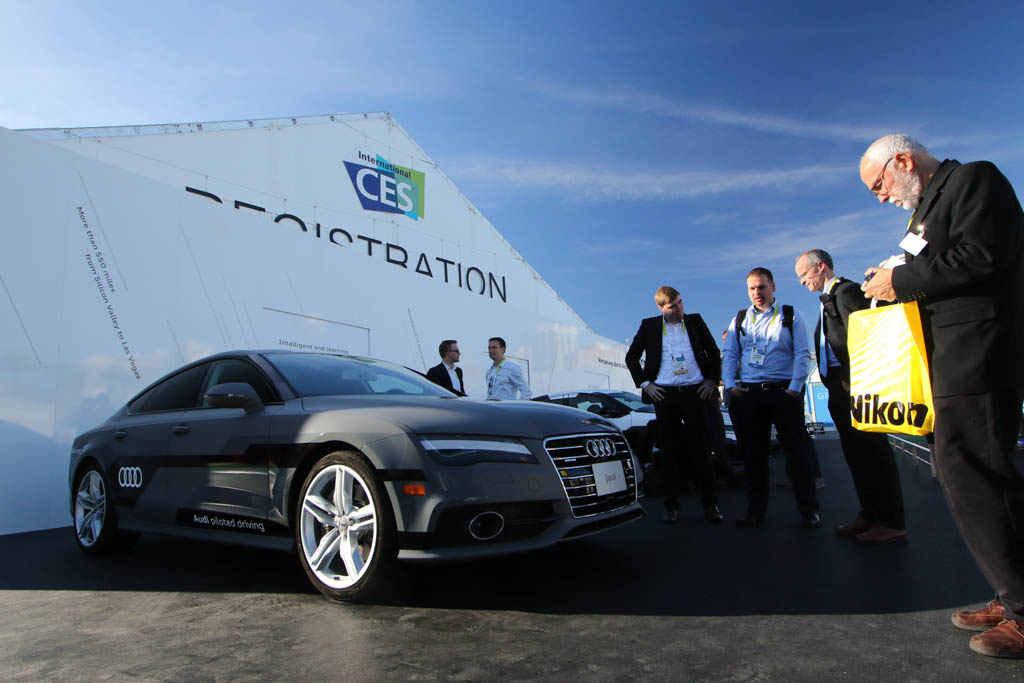
\includegraphics[width=0.8\textwidth]{images/150106_0345_ces.jpg}
	\captionsource{Audi A7 på 2015 CES.}{\url{https://a248.e.akamai.net/f/574/7105/8d/www.extremetech.com/wp-content/uploads/2015/01/150106\_0345\_ces.jpg}}
	\label{fig:Audi_A7}
\end{figure}
Audi viste deres A7 frem, hvilken af de tre ligner mest en almindelig personbil (se figur \ref{fig:Audi_A7}), men den kan selv køre over lange distancer. Hvis den dog opdager mange mennesker i et område, typisk hvis den kører imod en by, vil den bede personen bag rattet om at overtage styrringen. Bilen havde inden konferencen kørt med nye trafikkanter og journalister fra Silicon Valley til Las Vegas, en distance på omkring 900km, næsten uden input fra føreren og dette selvom bilen kørte 110km/t. Bilen benytter sig af sensorer som allerede bliver fabrikeret, som også er i stand til præcist at se bilens omgivelser. Sensorene inkluderer adaptiv fartkontrol, overvågning over blinde vinkler, varsling hvis du er ved at køre af vejen, tre typer sensorer som allerede bliver brugt i diverse fartøjer i dag. Desuden kommer bilen også med andre sensorer, så som laserscannere og kameraer, som gør bilen i stand til bedre at opdage objekter, både hvis objekterne er i bevægelse og hvis de er stillestående. Kameraerne som optager i 3D, hjælper bilen med at holde styr på omkringværende trafik. Bilen er i stand til at køre på veje, som ikke har høje bakker, hvor ingen biler pludseligt kører ind i din kørebane eller en bil foran panikbremser.

\subsubsubsection{Mercedes-Benz F 015}
Denne bil blev lavet, som et proof-of-concept og vil ikke blive sat i produktion, da udsynet for passagerne er alt for småt, men den indeholder teknologi og idéer, som ikke er set før. F 015 har LED på hver side af forenden, som hjælper fodgængere med at se om det er sikkert for dem at gå ud foran bilen --- en slags alternativ til fodgængerfelter og trafiklys i dag. Disse LED'er følger fodgængeren, mens han eller hun går forbi bilen og viser dermed at bilen har øje med dem. Disse LED'er kan ses på bilen på figur \ref{fig:Mercedes-Benz_F_015}.
\begin{figure}[h!]
	\centering
	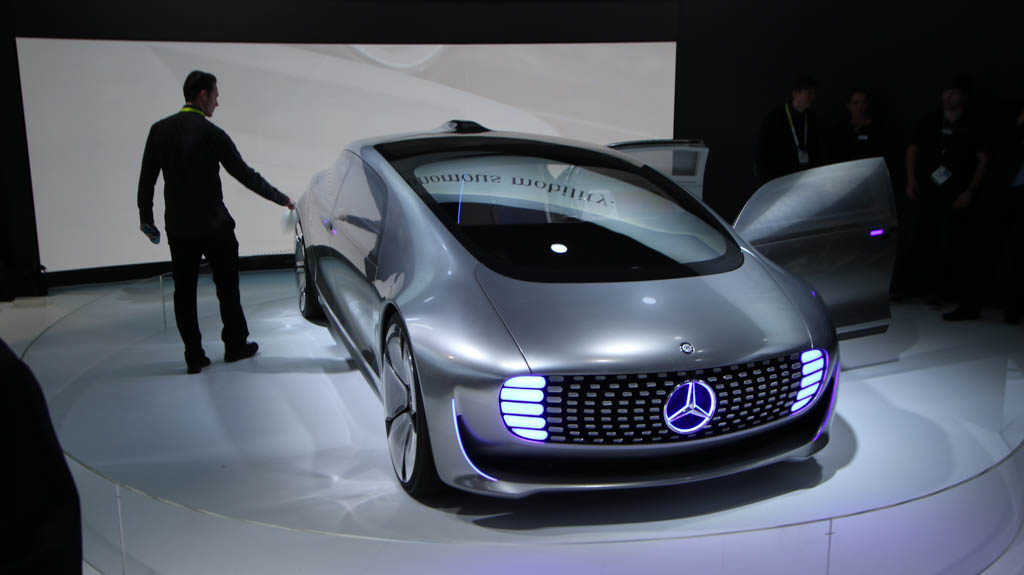
\includegraphics[width=0.8\textwidth]{images/150106_0422_ces.jpg}{}
	\captionsource{Mercedes-Benz konceptbilen F 015.}{\url{https://a248.e.akamai.net/f/574/7105/8d/www.extremetech.com/wp-content/uploads/2015/01/150106\_0422\_ces.jpg}}
	\label{fig:Mercedes-Benz_F_015}
\end{figure}
\FloatBarrier
Fodgængere kan potentielt krydse vejen, hvor de har lyst, hvis bilerne på vejen indikerer det er sikkert nok for dem. Forsæderne i bilen vender imod bagsæderne, hvilket gør alle folk i bilen i stand til at holde øjekontakt under samtaler. Sæderne har også mulighed for at rotere horisontalt, så passagerne nemt kan stige ind og ud af bilen.
\subsubsubsection{BMW i3}
BMW tog en eksisterende bil og modificerede den indenfor et helt bestemt område; parkering. Bilen på figur \ref{fig:BMW_i3} er i stand til, at parkere sig selv og ikke ligesom vi i dag kender det, hvor bilen parallelparkerer. Med BMW i3 kan man køre hen til indgangen til en parkeringsplads, gå ud af bilen og BMW i3 vil selv køre rundt på parkeringspladsen indtil den finder en fri plads. Herefter parkerer den selv, låser og slukker. Når man har brug for bilen igen, kan man inde i BMWs smartphone app til bilen tilkalde den og så bare vente ved indgangen til parkeringspladsen, hvor bilen selv vil køre hen og samle dig op. Ikke kun skal bilen være i stand til at navigere rundt, den skal også være i stand til at undgå andre bilister, parkerede biler og ikke parkere på parkeringspladser prioriteret til handicappede.
\FloatBarrier
\begin{figure}[h!]
	\centering
	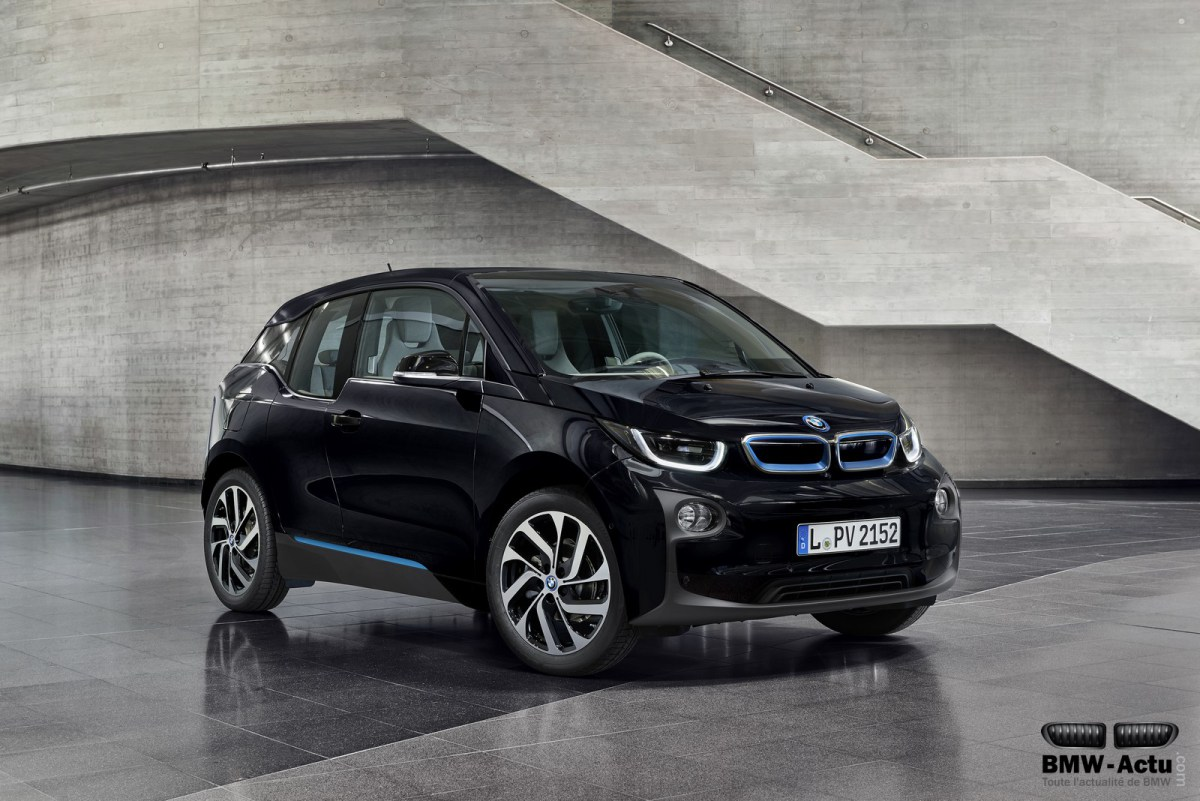
\includegraphics[width=0.8\textwidth]{images/bmw-i3-fluid-black-1.jpg}
	\captionsource{Den selv-parkerende BMW i3.}{\url{https://bmwactu.files.wordpress.com/2015/09/bmw-i3-fluid-black-1.jpg}}
	\label{fig:BMW_i3}
\end{figure}
\FloatBarrier
	\subsection{Samfundsmæssige}
	I dette delafsnit vil vi fokusere på de samfundsmæssige problemer i forhold til de selvkørende biler. Disse problemer er problemer som politikkerne skal tage stilling til, samt problemer som kunne skræmme eventuelle købere væk.
	\subsubsection{Robotetik}
	Når der snakkes om selvkørende biler, bliver der ofte stillet etiske spørgsmål. Når man overfører kontrollen over bilen fra mennesket, og overgiver dette til bilen selv, overføres også et stort ansvar. I tilfælde af at bilen kommer ud for et uheld, hvad skal bilen så gøre? Der er mange muligheder, men de kan ligeledes alle have store konsekvenser. Hvis en person ender foran bilen, skal den kunne træffe en beslutning om at forsøge at undvige personen, og køre galt, eller om den blot skal forsøge at bremse. Hvis bilen bremser, er det ikke sikkert at bilen kan nå at bremse før personen, men hvis den forsøger at undvige er det muligt at den kører sammen med en modkørende bil. 

	Alt efter bilens programmering ville den kunne forsøge at minimere skader, ved at træffe det valg der vil forårsage færrest menneskeskader. Men dette kunne bringe uskyldige mennesker i fare, hvis bilen valgte at undvige en person ved at køre over i den anden side af vejen, hvor en modkørende bil kunne befinde sig. 
	
	Dette er spørgsmål som endnu ikke er besvaret fra de selvkørende biler, da dagens biler i en sådan situation vil overlade styringen til føreren. En undersøgelse (se figur \ref{fig:etik_accident}) blev i 2014 foretaget af Open Roboethics Initiative, hvor mennesker blev adspurgt om hvordan de ønskede at bilen skulle opføre sig i en situation som nævnt ovenfor. 52\% af de adspurgte mennesker ønsker at bilen skal forsøge at minimere skaderne ved at fordele disse mellem både passagerer og fodgængere. 
	\begin{figure}[h!]
		\centering
		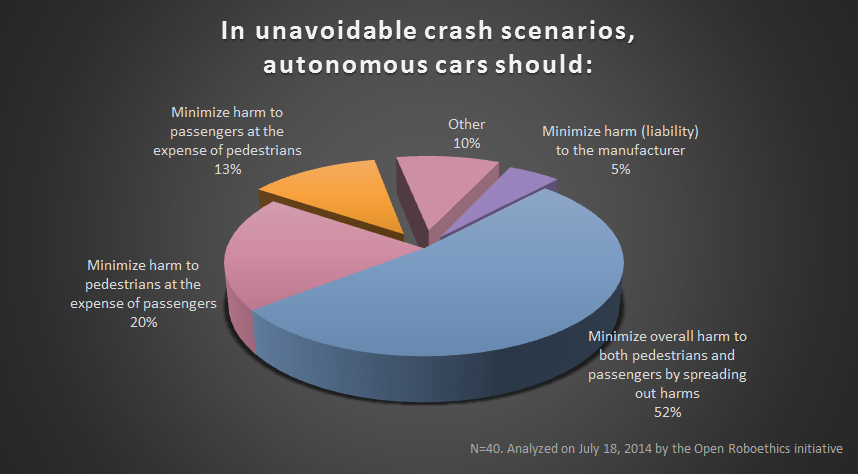
\includegraphics[width=\textwidth]{images/roboethics-2.jpg}
		\captionsource{Undersøgelse om hvad folk vil foretrække i en uundgåelig ulykke}{\url{http://www.openroboethics.org/results-random-chance-over-informed-decision/}}
		\label{fig:etik_accident}
	\end{figure}
	
	 I et scenarium hvor et tog kommer kørende ned ad en bane imod tre mennesker spændt fast til togskinnerne, men inden toget støder mod disse tre personer, er der et baneskift. Hvis der på den anden række togskinner kun ligger \'en person, vil den logiske løsning være at skifte bane for toget, da der dermed reddes 2 menneskeliv. Men hvad hvis denne ene person er meget betydningsfuld for en, så som en mor, eller ens egen søn, ville samme person så træffe samme valg, og vælge at slå sit eget barn ihjel, frem for tre fremmede mennesker? En maskine vil stadig tænke logisk og træffe samme valg da færre liv går tabt, men ingen forældre vil have det komfortabelt med at benytte en bil, som kan træffe selv samme beslutning og slå deres eget barn ihjel som muligvis sidder på bagsædet, frem for at ramme nogle fremmede fodgængere.
	
	Tilbage i 1942, præsenterede science fiction forfatteren Isaac Asimov, 3 gyldne love\cite{Asimov}, som siden er blevet brugt utallige gange til at beskrive hvordan en robot hovedsageligt skal omgås mennesker.
	
	\begin{enumerate}
		
		\item En robot må ikke gøre et menneske fortræd, eller, ved ikke at gøre noget, lade et menneske komme til skade
		\item En robot skal adlyde ordrer givet af mennesker, så længe disse ikke er i konflikt med første lov
		\item En robot skal beskytte sin egen eksistens, så længe dette ikke er i konflikt med første eller anden lov
		
	\end{enumerate}
	
	Disse tre love er i bund og grund også etiske, da de siger at robotten ikke må adlyde et menneskes ordre hvis dette forårsager skader på andre mennesker, men samtidig skal sørge for mennesker ikke kommer til skade. Hvis et deprimeret individ springer ud foran en selvkørende bil i et forsøg på at begå selvmord, må bilen ikke bare køre personen over, da dette er i strid mod første lov. Bilen bliver derfor nødt til at undvige, også selvom dette kan totalskade bilen, og brække et legeme eller to på passageren, da et brækket ben er langt bedre end et mistet liv, samtidig med at overholde Asimov's 3 love. Her bliver føreren af bilen dog ``straffet'' for at et andet menneske forsøger at tage sit eget liv. Skal bilen i dette tilfælde gøre det samme som føreren af en manuelt-kørende bil og køre ham ned da det er umuligt at undvige, selvom dette vil være i strid mod første lov? 

	Det kan være svært at svare på disse spørgsmål, og i sidste ende vil sådan nogle problemstillinger besvares ved at politikere fastsætte love der giver producenterne nogle klare linjer at programmere efter.
	\subsection{Teknologiens effekt}
Da de selvkørende biler som navnet antyder selv kører, bliver der i den forbindelse selvfølgelig skrevet en del kode til dem for at sikre at de kører ordentligt i trafikken. Dette betyder at bilen overholder de forskellige færdselslove, hvilket i sig selv er godt nok, men dette vil også have nogle seriøse økonomiske konsekvenser blandt andet for det offentlige men også for de mange private virksomheder. 

Mange af de problemer de selvkørende biler skaber kan finde hos den offentlige sektor. Det er som udgangspunkt meget lige til at finde ud af hvordan de vil påvirke politiet og den indkomst staten har derfra, da den selvkørende bil er programmeret til at overholde trafiklovene, betyder det at der vil blive uddelt færre bøder. Politiet vil derfor komme til at have en lavere indtjening, da en stor del af denne nemlig kommer fra uddeling af bøder\cite{B}. Der vil heller ikke være brug for lige så mange betjente rundt omkring i landene, især ikke hvis alle biler bliver erstattet a selvkørende. Dette er fra statens side positivt da det betyder at der er færre der skal have løn, men det betyder derfor også at der kommer flere arbejdsløse hvilket er dårligt for økonomien.

Udover staten vil mange private virksomheder, som for eksempel taxier, lastbiler og mange andre former for transport, også kunne mærke denne ændring til selvkørende biler. Man er allerede i New York bgyndt at eksperimentere med selvkørende taxier, hvilket for firmaerne både kan spare tid og penge. De regner eksempelvis med at indføre 5.000 selvkørende taxier i 2016, hvilket også vil betyde at man kan forvente 5.000 arbejdsløse mere på gaderne i New York. Derudover er der selvfølgelig også lastbilerne som transportere en masse forskellige varer rundt omkring over alt i verden. Dette kan nemlig også gøres ved hjælp af selvkørende biler, heraf lastbiler. Man bruger allerede halvt selvkørende lastbiler, hvilket gør det muligt at fjerne hænderne fra rettet på motor vejen, og det burde ikke vare længe før der slet ikke er brug for nogle bag rettet

Et sidste område hvor ændringen til selvkørende biler vil skabe problemer er for de mange tankstationer og andre sælgere at de fossile brændsler. De selvkørende biler vil nemlig uden tvivl være elektriske, hvilket vil ødelægge markedet for fossile brændsler, men også skabe en del arbejdsløse i forbindelse med arbejderne på de forskellige boringsplatformer til de unge der står bag disken på den lokale tankstation.

\subsubsection{Links (vil blive flyttet senere til literaturlisten)}
http://inhabitat.com/nyc/google-signs-agreement-with-nyc-mayor-to-replace-nyc-taxis-with-driverless-google-cabs/ 
http://sand.blogs.business.dk/2015/08/18/google-car-og-dens-ligesindede-vil-smadre-supermarkeder-benzinstationer-og-faerdselsbetjente/


Andre links:
http://zackkanter.com/2015/01/23/how-ubers-autonomous-cars-will-destroy-10-million-jobs-by-2025/
http://www.washingtonpost.com/news/innovations/wp/2015/07/07/sorry-but-the-jobless-future-isnt-a-luddite-fallacy/
http://sand.blogs.business.dk/2015/08/18/google-car-og-dens-ligesindede-vil-smadre-supermarkeder-benzinstationer-og-faerdselsbetjente/
http://www.computerworld.dk/art/234200/her-er-udfordringerne-med-selvkoerende-robotbiler-i-danmark

	\section{Problemafgrænsning}
	\textit{I dette afsnit vil vi indsnævre vores problemrum fra problemanalysen, og finde frem til fokusområde for vores problemformulering, og for en eventuel løsning af et af problemerne vi har fundet i problemanalysen. Ud fra denne problemafgrænsning, vil vi så opstille en problemformulering.}.
    \label{afgraensning}
\subsection{Valg af fokusområde}
I vores problemanalyse har vi kigget på de teknologiske og samfundsmæssige problemer omkring teknologien. Der har været problemer af begge typer, men de problemer som har vist sig i form af ulykker for bilen, har været fordi bilen ikke har kørt som andre mennesker. Som nævnt i afsnit \ref{interaktion}, kører den selvkørende bil blandt andet ikke aggressivt nok, hvilket har forårsaget at biler er kørt op bag i den.

\subsection{Bilens syn}
Så hvordan undersøger bilen hvad der er rundt om den? Både Tesla og Audi benytter sig af Nvidia Drive PX, hvilket er en udviklingsplatform, som tillader bilen det er installeret i, at tilgå Nvidias nye deep-learning platform kaldet DIGITS. Dette gør det muligt for enheder, at lære deres omgivelser at kende, og er designet til at fungere ligesom et menneske. 

\begin{figure}[h!]
	\centering
	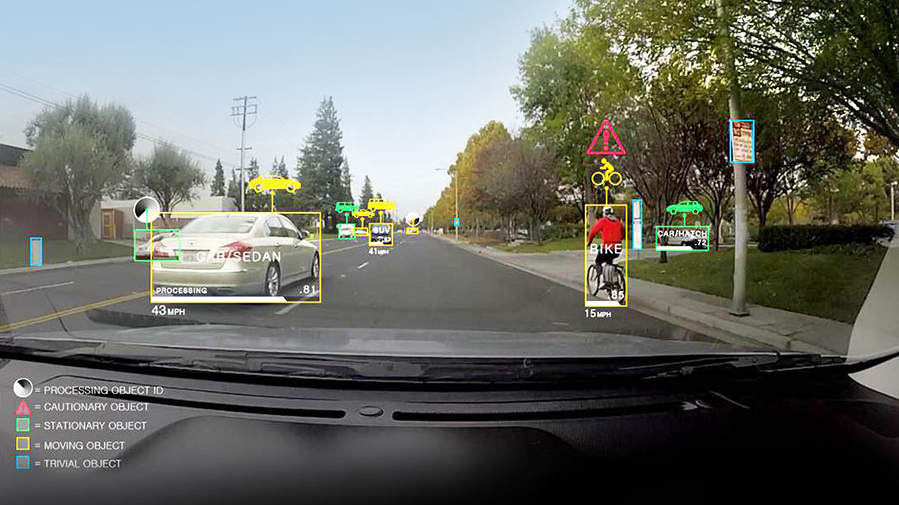
\includegraphics[width=\textwidth]{images/nvidiadrive.png}
	\captionsource{Nvidia DRIVE PX analyserer omgivelserne, og kan inddele objekter i forskellige grupper.}{\url{https://www.nvidia.com/object/drive-px.html}}
	\label{fig:DRIVE}
\end{figure}
Ligesom mennesker lærer med tiden og af deres erfaringer, vil bilerne også lære af deres erfaringer, men da de alle er koblet til dette netværk, lærer alle bilerne, af alle bilers erfaringer \cite{Nvidia}. Dette board uploader sine data til DIGITS, og hvis der er noget indsamlet data den ikke er sikker på hvad den skal gøre med, vil dette data blive kigget og regnet på af hele netværket.

DIGITS analyserer billeder fra kamerarer rundt om bilen, og inddeler objekterne rundt om bilen i klasser. På figur \ref{fig:DRIVE} kan man se hvordan objekter er klassificeret på et stilbillede.

DIGITS er selvfølgelig kun \'en platform, og andre producenter af selvkørende biler vil måske benytte sig af andre systemer. Men det vigtigste er blot at kunne skille de forskellige objekter fra hinanden \cite{cnet}, så ikke alt ses som den samme type objekter. Grunden til dette er, at bilen skal kunne forholde sig anderledes over for en cyklist, end for en anden bil. Programmet bliver nødt til at kende forskellen på en parkeret bil der holder i vejkanten, og en bil som kommer fra en sidevej og kan finde på at køre ud foran den selvkørende bil. Normaltvist vil et menneske forsøge at få øjenkontakt med en billist som kommer fra en sidevej, for at sikre sig at bilen er blevet set, men da en selvkørende bil ikke kan lave øjenkontakt, bliver den nødt til at kunne adskille de forskellige typer af objekter på vejene.

\subsection{Typer af trafikanter}
Det er vigtigt at en selvkørende bil kan adskille forskellige typer af trafikanter, da de hver især har forskellige karakteristika. I en rapport fra Havarikommissionen for vejtrafikulykker viser resultaterne, at størstedelen af de ulykker der skete mellem cyklister og billister skyldtes dårlige trafikvaner \cite{HVU}. I 17 ud af 30 undersøgte ulykker havde cyklisten vigepligt, men kørte alligevel ud i krydset. Undersøgelsen konkluderer at både cyklister og billister var opmærksomme, og at ulykkerne overvejende skyldtes dårlige trafikvaner. 

Hvad betyder det så for de selvkørende biler? Det betyder at hvis bilen opdager en cyklist, bliver den nødt til at vide at nogle cyklister har dårlige trafikvaner, og at den derfor skal være opmærksom på at cyklisten ikke nødvendigvis vil køre efter de gældende trafikregler. 

For motorcykler er det dog et andet problem der skal tages hensyn til.  I en undersøgelse fra Havarikommisionen offentliggøres det at ud af 41 ulykker vedrørende motorcykler, kunne halvdelen af ulykkerne være undgået hvis motorcyklisten havde haft en mere moderat hastighed \cite{MOT}. For den selvkørende bil kan dette også have en betydning, hvor den skal til at tænke over om motorcyklister har for høj en fart, og hvordan den skal reagere i forhold til en eventuel forhøjet fart.

I forhold til billister har vi allerede i afsnit \ref{interaktion} set på eksempler, hvor folk er kørt ind i Googles selvkørende bil, fordi den er bremset op til et gult lys. Bilen skal derfor være i stand til forudsige om bilen bagved vil stoppe. For hvis den selvkørende bil kan nå over lyskrydset inden det bliver rødt, vil dette være at foretrække frem for at være i fare for at bilen bagved kører op i den selvkørende bil.

Til sidst har vi så fodgængerne, som skal tages hensyn til. Bilen skal kunne kende forskel på en voksen og et barn, da der skal køres mere forsigtigt omkring børn. Fodgængere skal altså kunne klassificeres i forhold til hvor ``uberegnelige'' de er. 	
    \section{Problemformulering}
	\bibliographystyle{plain}
	\bibliography{sources}
\end{document}